\chapter[Jugement délibéré, les régimes alimentaires]{Jugement délibéré, les régimes alimentaires\raisebox{.3\baselineskip}{\normalsize\footnotemark}}
\footnotetext{\url{https://github.com/barnabegeffroy/vegan_or_not}}
Ce projet a pour but de mettre en pratique les théories exposées dans l'article \textit{A formal framework for deliberated judgment}\cite{cailloux_formal_2020}. Cette article de théorie du choix s'intéresse à l'influence des arguments dans la prise de décision. Le jugement délibéré est le fait de prendre une décision en ayant pris en compte différents arguments qui ne vous feront pas changer d'avis. Pour avoir des données empiriques sur ce modèle, il a été convenu de s'intéresser aux régimes alimentaires proposés dans une cantine.

\section{Protocole de l'expérience}
L'idée est de proposer aux utilisateurs un site web sur lequel l'influence des arguments dans leur assentiment à une cantine végane ou non est suivie. Pour cela le site web proposera des vidéos de deux experts, un en faveur des régimes véganes, l'autre contre ce genre de régimes alimentaires. L'utilisateur aura accès à une bibliothèque de vidéos d'arguments des deux experts. Cette bibliothèque sera dynamique et évoluera en fonction des vidéos vues. Si l'utilisateur a vu l'argument 1 de l'expert A, il aura alors accès à la réponse de l'expert B, le contre-argument. Si ensuite, il visionne ce contre-argument, il aura accès au contre-contre-argument de l'expert A, et ainsi de suite jusqu'à ce que le débat sur cet argument soit clos par l'un des experts. Le site web doit également proposer des formulaires, en fonction des vidéos visionnées, afin de capturer la tendance de l'opinion de l'utilisateur et le moment où celui-ci émettra un jugement délibéré. Ces formulaires permettront d'étudier la puissance des arguments des deux experts et la tendance des utilisateurs dans leur prise de décision. Outre ces formulaires, le site web doit fournir des informations techniques sur le parcours de l'utilisateur, notamment le temps de visionnage des différentes vidéos.

\section{Création d'un site web}
Le site web doit répondre aux exigences du protocole : 
\begin{itemize}
    \item proposer une bibliothèque de vidéos dynamique.
    \item fournir des formulaires adaptés aux vidéos visionnées.
    \item récupérer les données de l'utilisateur sur le visionnage des vidéos.
\end{itemize}
En ce qui concerne le premier et dernier point, ils sont fortement liés. En effet, une fonction pourrait permettre de débloquer la réponse à un argument une fois que l'information "vidéo lue jusqu'à la fin" serait transmise. Pour réaliser cela, \textit{video.js}, lecteur open source, permet d'obtenir de nombreuses données nécessaires pour le projet.

Ce projet a été réalisé avec une étudiante en nutrition, il fallait alors également trouver une interface opensource permettant d'éditer un site web facilement.

\subsection{WordPress}
WordPress est un logiciel de conception web (CMS). Il est utilisé par 35\% des sites web dans le monde. WordPress permet de réaliser un site web de qualité sans avoir besoin de compétences techniques importantes (HTML, JavaScript). Il propose différents modèles adaptables facilement et plus de 30 000 extensions permettant d'accéder facilement à de multiples fonctionnalités (vidéos, formulaires, analyse de fréquentations, ...). WordPress semble ainsi être l'interface opensource parfaite pour éditer le site web facilement tout en respectant le protocole.

\begin{figure}[!ht]
    \begin{center}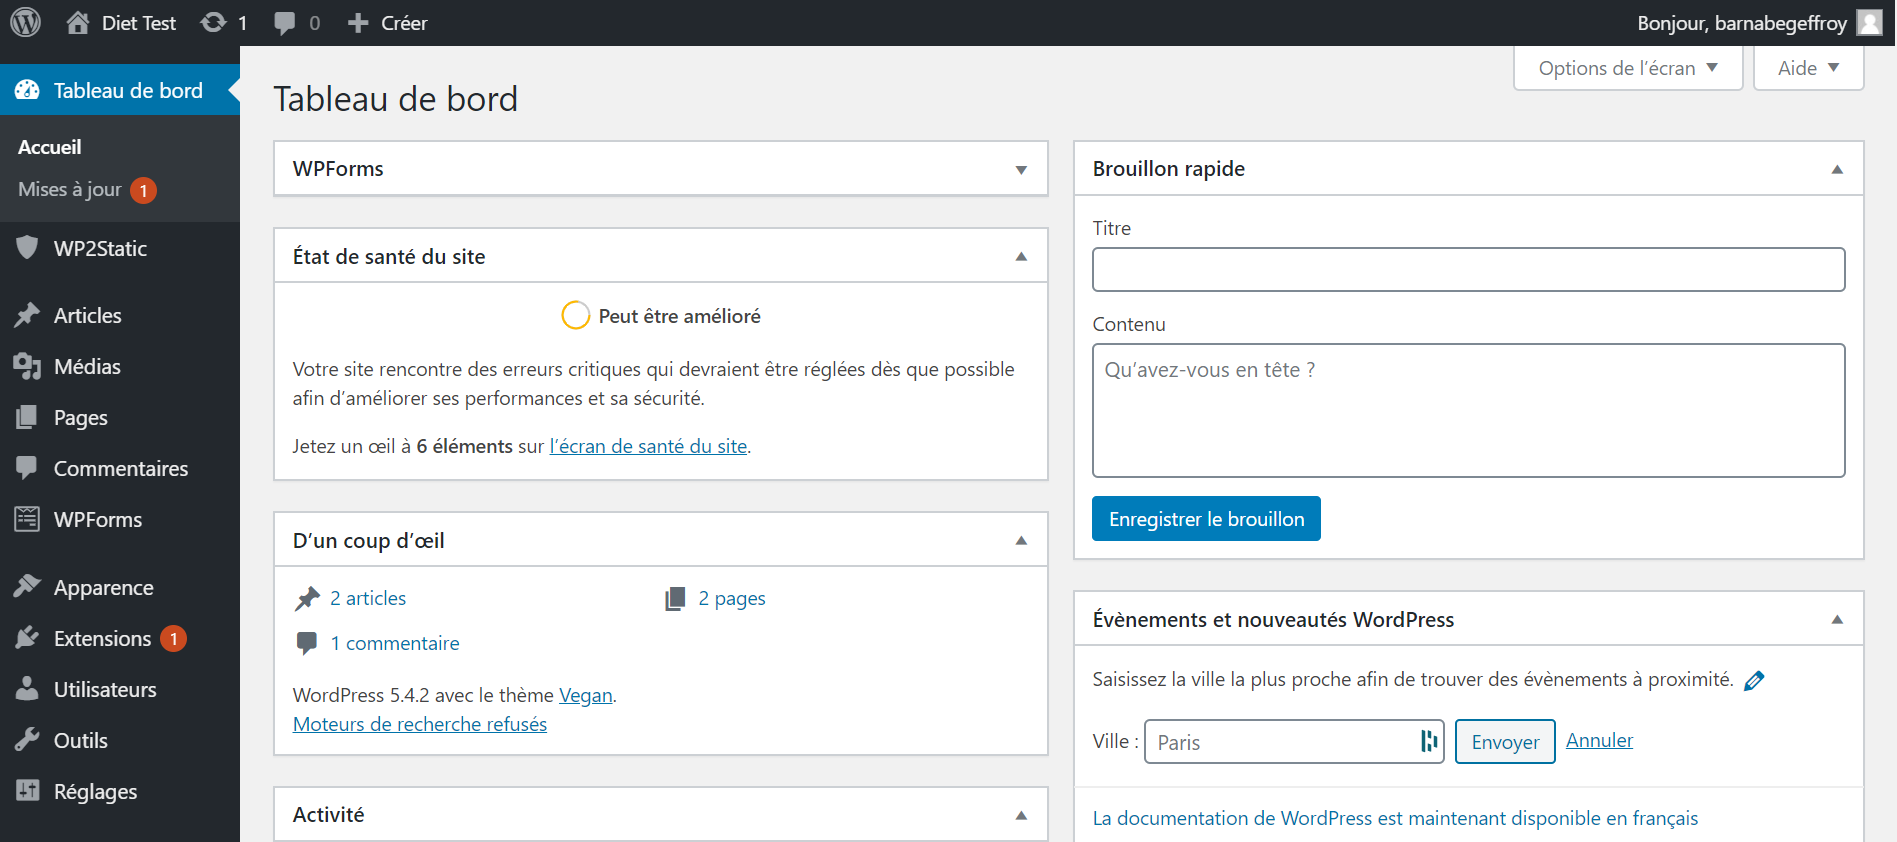
\includegraphics[width=\textwidth]{assets/wp.PNG}
    \end{center}
    \caption{Capture d'écran de l'interface de WordPress}
\end{figure}
Une contrainte s'ajoutait tout de même en utilisant WordPress. Le fait de dépendre d'extensions pouvant évoluer et ne plus être compatible avec nos exigeances était en effet un risque à éviter. De plus, le code source est très peu accessible sur WordPress, il est très compliqué de réaliser un site web sur mesure lorsque celui-ci exige des points techniques très précis.

Il a donc été décidé de concevoir l'esthétique du site sur WordPress (affichage, thème, polices, images). La partie technique (dynamisme, récupération des données) serait développée sur Jekyll.

\subsection{Jekyll}
\subsubsection{Fonctionnement}
Jekyll est un générateur de site statique\footnote{Une page web statique est une page web dont le contenu ne varie pas en fonction des caractéristiques de la demande.}. Ce logiciel permet de générer facilement une architecture web convaincante. Jekyll propose un système de modèle de page. Celui-ci permet d'obtenir des pages suivant les mêmes caractéristiques (styles, en-tête, pied de page, barre de navigation, ...) sans recopier sur chaque page le code HTML nécessaire. Le code permet également la conversion de fichier Markdown\footnote{Markdown est un langage de balisage offrant une syntaxe facile à lire et à écrire.}, éditable facilement, en page HTML. Chaque fichier doit er par une en-tête lue par Jekyll (voir ci-dessous). Celle-ci contient les informations permettant à Jekyll de générer une page HTML. Le fichier ne peut contenir que cette en-tête, comme ci-dessous.
\begin{figure}[!ht]
\begin{lstlisting}[language=Ruby]
---
layout: post
title:  "Le premier argmuent de l'expert A!"
date:   2020-03-27
excerpt: "S1a"
image : {{page.image}}
---
\end{lstlisting}
\caption*{Contenu d'un fichier suivant le modèle \texttt{post} pour générer une page vidéo}
\end{figure}

Jekyll va, en suivant ces quelques lignes suivrent, générer la page web (voir figure~\ref{s1a}) à partir du modèles post. L'annexe~\ref{sec:shtml} détaille le code HTML généré par Jekyll et permet de se rendre compte de l'efficacité de Jekyll, seulement sept lignes de code ont suffit à générer 190 lignes de code HTML. La page contient une vidéo qui est généré par l'\texttt{excerpt} (l.72 à 75).

\vspace{1cm}
\begin{figure}[!ht]
    \begin{center}
        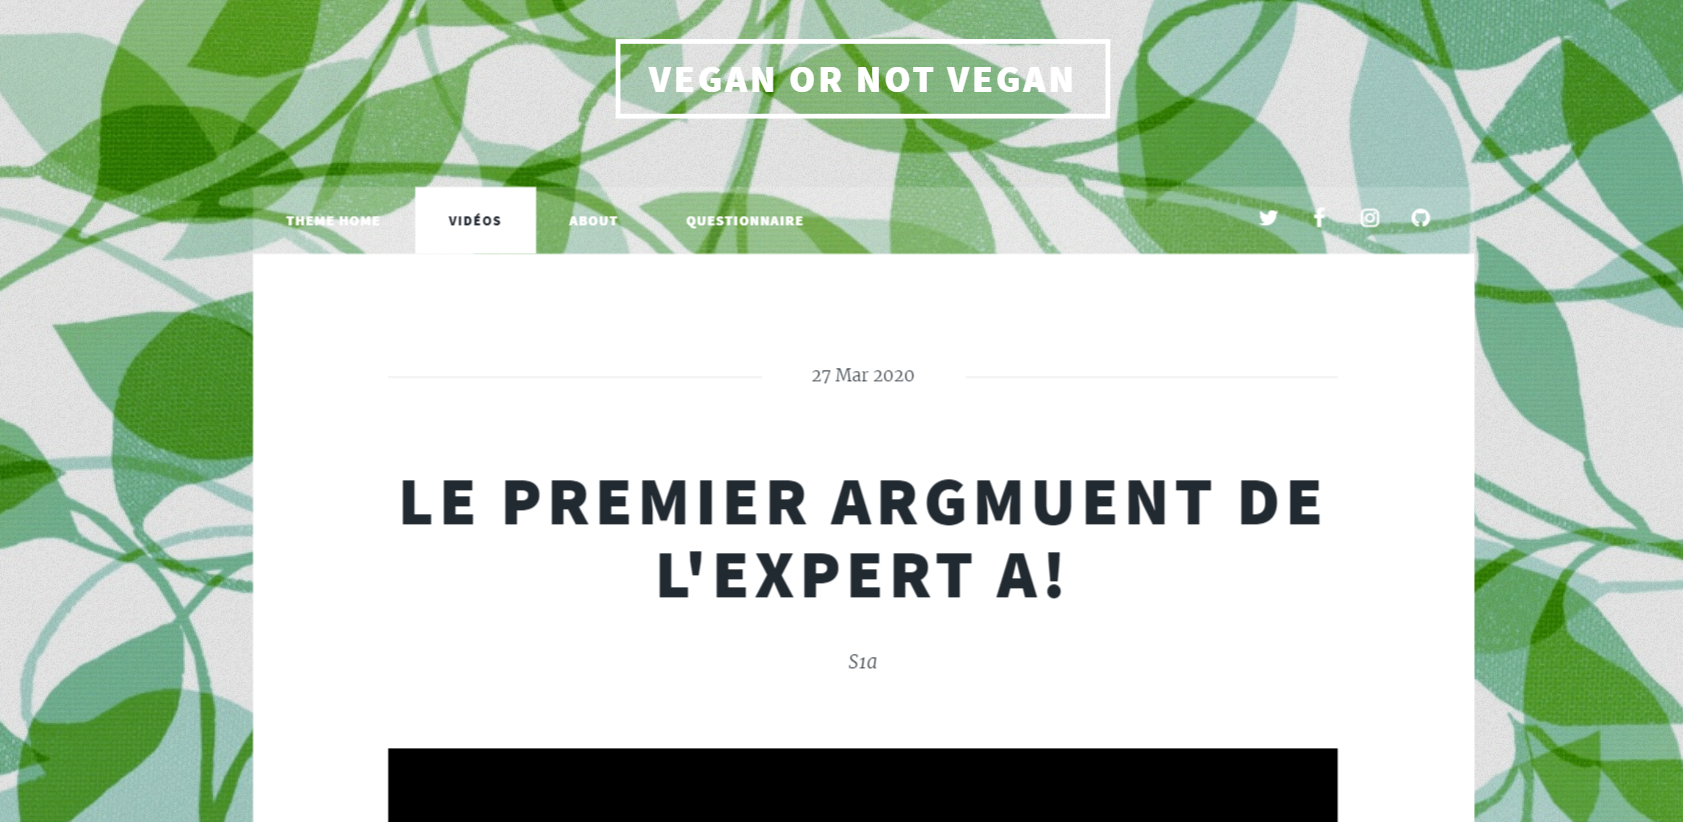
\includegraphics[width=0.8\textwidth]{assets/s1a.PNG}
        \caption{Capture d'écran de la page web généré par les lignes de codes ci-dessus}
        \label{s1a}
    \end{center}
\end{figure}

\subsubsection{Thèmes}
Jekyll possède une bibliothèque de thème opensource avec des nombreux modèles préexistants. Le thème de la figure~\ref{s1a} avait d'abord été choisi en attendant de récuprer les données esthétiques du site WordPress. Cependant ce thème présentait quelques disfonctionnements et le thème de la figure a finalement été choisi

\begin{figure}[!h]
    \begin{center}
    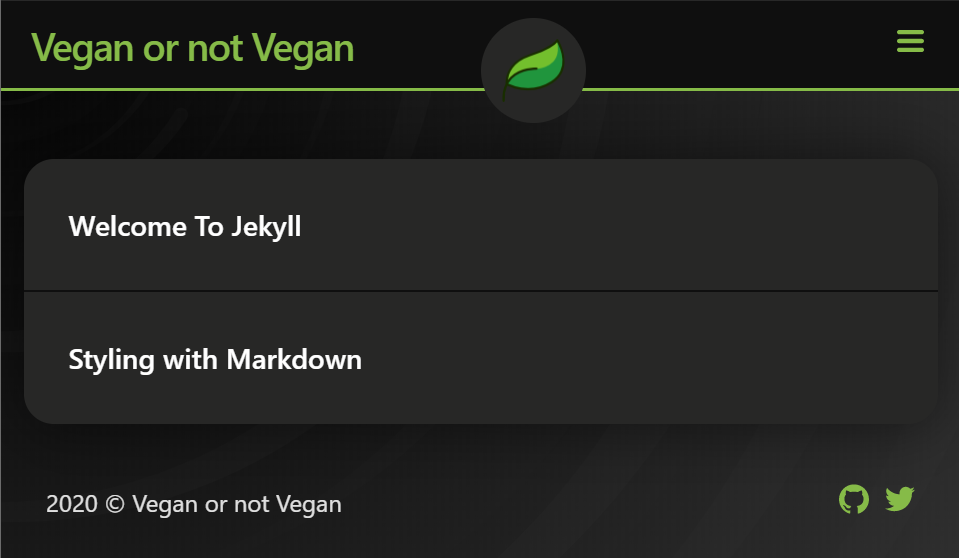
\includegraphics[width=0.7\textwidth]{assets/newtheme.PNG}
    \end{center}
    \caption{Nouveau thème Jekyll utilisé provisoirement dans l'attente de l'esthétique WordPress}
\end{figure}

\section{Déploiement sur Internet}
\subsection{Jekyll}
Jekyll a été créé par le fondateur de GitHub, Tom Preston-Werner. Son déploiement sur Jekyll est relativement simple. Il suffit de déposer les fichiers générés par Jekyll sur un dépôt GitHub pour que ceux-ci soient déployés sur un site web, une page GitHub.

La génération des fichiers par Jekyll est automatisé de la même manière que plaquette-MIDO avec Travis-CI (voir section~\ref{sec:automatisation}). Le dépôt vers lequel les fichiers sont déployés est \href{https://github.com/barnabegeffroy/vegan_or_not}{\textcolor{blue}{\underline{vegan\_or\_not}}}. GitHub va donc créer une page GitHub à partir du contenu de ce dépôt. On obtient ainsi notre site web, \href{https://barnabegeffroy.github.io/vegan_or_not/}{\textcolor{blue}{\underline{Vegan or not vegan}}}.

\subsection{WordPress}
Le déploiement de la page WordPress sur Internet est un peu plus complexe. Pour un déploiement optimal, WordPress préconise de passer par un hébergeur web adapté et payant. Une extension WordPress existe cepandant pour convertir le contenu WordPress en statique, lisible par GitHub pour générer une page GitHub. Cette extension s'appelle WP2Static. Elle crée un répertoire contenant les fichiers statiques. Il suffit de pousser ces derniers vers un dépôt GitHub pour que le site web soit déployé. Un exemple de page WordPress déployé sur une page GitHub est disponible sur ce \href{https://barnabegeffroy.github.io/static-wp/}{\textcolor{blue}{\underline{lien}}}.